\chapter{Marco de referencíal}

\section{Marco teórico}


\subsection{Tipos de gallinas}

La gallina de engorde y la gallina de postura \index{gallina de postura} son dos tipos de aves de corral que se crían con diferentes propósitos en la industria avícola.
La gallina de engorde se cría para producir carne en un período de tiempo corto, generalmente alrededor de 6 semanas, mientras que la gallina de postura se cría para producir huevos durante un período de tiempo más prolongado, generalmente alrededor de 1-2 años.

La alimentación y el manejo de estas aves varían según su propósito de producción. La nutrición de la gallina de engorde se enfoca en maximizar su tasa de crecimiento y conversión alimenticia, mientras que la gallina de postura requiere una dieta adecuada para mantener una producción de huevos sostenible y saludable.

La Hy-Line Brown \cite{Hy-Line} imagen \ref{fig:Gallina Hy-Line}, es la ponedora de huevo marrón mejor balanceada. Produce huevos color marrón oscuro hasta las 100 semanas. Su guía de manejo indica la cantidad adecuada de alimento al día que debe consumir cada gallina de acuerdo a la semana de vida en la que se encuentre.

\begin{figure}[htpb]
    \centering
    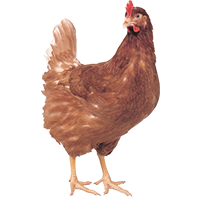
\includegraphics[width=0.4\linewidth]{imagenes/imacap/marcoteo/Hy-Line Brown.png}
    \caption{Gallina Hy-Line Brown}
    \label{fig:Gallina Hy-Line}
\end{figure}

\subsection{Sistemas de producción}\index{sistemas de producción}

La publicación de SAGARPA “Situación actual y perspectiva de la producción de carne de pollo en México 1990- 1997”, establece que en México existen tres sistemas de producción basados en el esquema tecnológico que utilizan:

\begin{enumerate}
    \item \textbf{Tecnificado}: \index{sistemas de producción!tecnificado} Se considera tecnificado a todo aquel sistema que utilice los adelantos tecnológicos disponibles a nivel mundial, principalmente grandes compañías y consorcios son quienes tienen estos sistemas. En donde se industrializan los procesos, aumentando la producción y rentabilidad del sistema.
    \item \textbf{Semi-tecnificado}: \index{sistemas de producción!semi-tecnificado} Cuentan con diferente grado de tecnificación y se encuentran en un punto medio entre un sistema tecnificado y un sistema rural. La producción es menor, aunque la calidad es similar a la que se encuentra en un sistema tecnificado.
    \item \textbf{Rural o traspatio}: \index{sistemas de producción!traspatio} Esquema productivo tradicional, su producción es muy baja.
\end{enumerate}

Mientras que, en sitios como Veterinaria Digital \cite{veterinaria-digital-sa-2024} y Avicultura.mx \cite{Avicultura} se proponen diferentes nombres. En veterinaria digital se les propone como:

\begin{enumerate}
    \item Intensivo o Jaula
    \item Semi intensivo
    \item Extensivo o Pastoreo
\end{enumerate}

Variando únicamente los nombres, manteniendo la definición, en este trabajo se opta por utilizar los nombres otorgados por la SAGARPA. En la imagen \ref{fig:Ejemplo Sitema Tec} se puede ver un sistema tecnificado que utiliza recursos tecnológicos para aumentar su eficiencia; foto perteneciente a \cite{Artabas}.

\begin{figure}[htbp]
    \centering
    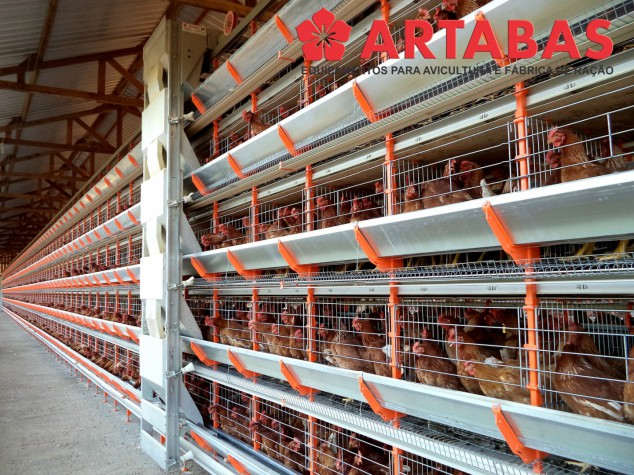
\includegraphics[width=0.75\linewidth]{imagenes/imacap/marcoteo/artabas-jaulas-ponedoras04-2.jpg}
    \caption{Ejemplo de un sistema tecnificado}
    \label{fig:Ejemplo Sitema Tec}
\end{figure}

\subsection{Sistemas de alimentación}

Los sistemas de alimentación \index{sistema de alimentación} para gallinas de postura son un elemento clave en la producción avícola. La alimentación adecuada de las aves es fundamental para su salud, bienestar y producción de huevos. A continuación, se presenta un marco teórico que describe los principales sistemas de alimentación para gallinas de postura.

\begin{enumerate}
    \item \textbf{Sistema de alimentación manual}: \index{sistema de alimentación!manual} este sistema consiste en la alimentación manual de las aves por parte del personal de la granja. Es el sistema más simple y económico, pero también el más laborioso. Requiere que el personal se encargue de la alimentación y el suministro de agua a las aves varias veces al día.
    \item \textbf{Sistema de alimentación por gravedad}: \index{sistema de alimentación!por gravedad} este sistema utiliza un dispensador de alimento que se llena periódicamente y que se encuentra suspendido sobre las jaulas o corrales de las aves. El alimento se dispensa automáticamente en los comederos de las jaulas a medida que las aves lo consumen. Este sistema es menos laborioso que el manual, pero requiere una supervisión periódica para asegurarse de que el dispensador esté lleno y funcionando correctamente.
    \item \textbf{Sistema de alimentación automático}: \index{sistema de alimentación!automático} este sistema es el más avanzado y tecnológico. Utiliza un controlador automático para dispensar la cantidad adecuada de alimento a las aves en momentos específicos del día. El sistema también puede incluir sensores para monitorear el consumo de alimento y agua de las aves, y ajustar automáticamente la cantidad dispensada en función de sus necesidades.
\end{enumerate}

Además, es importante tener en cuenta la composición y calidad del alimento. Las gallinas de postura requieren una dieta equilibrada y rica en proteínas, vitaminas y minerales para mantener una buena salud y producir huevos de alta calidad. Por lo tanto, los sistemas de alimentación deben estar diseñados para suministrar una dieta adecuada y adaptada a las necesidades de las aves.

\subsection{Nidal}

El nidal \index{nidal}, imagen \ref{fig:EjNid}, es el espacio en que la gallina pone sus huevos; su tipo, tamaño, ubicación y limpieza son aspectos fundamentales a tener en cuenta.\cite{unknown-author-2024}

\begin{figure}[htbp]
    \centering
    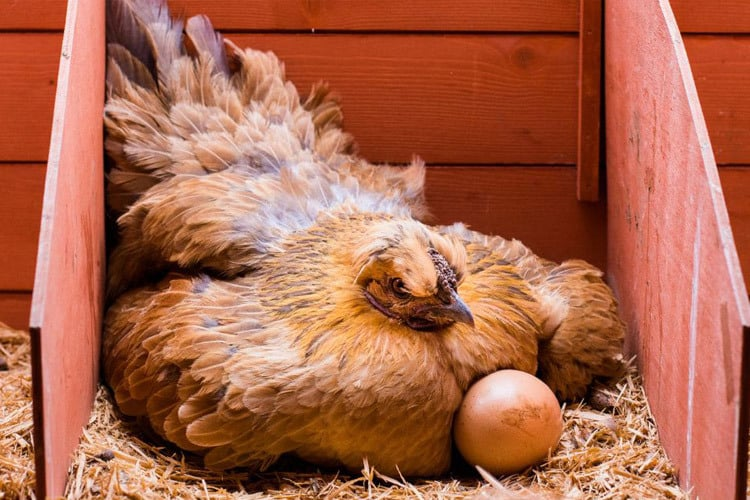
\includegraphics[width=0.75\linewidth]{imagenes/imacap/marcoteo/Nidal.jpg}
    \caption{Ejemplo de un nidal}
    \label{fig:EjNid}
\end{figure}

La ubicación de los nidales es importante, por lo que deben localizarse en un lugar tranquilo y con fácil acceso, para que las aves se encuentren libres de estrés. \cite{agrinews-2016}

La cantidad de nidales dependerá de la cantidad de gallinas, pero en general se recomienda que por cada metro cuadrado de nidal útil existan entre 100 y 200 aves.

Otra característica importante es el suelo del nidal. Es necesario prestar atención a las medidas higiénicas, buscando un suelo atractivo. Se busca la máxima simplicidad estructural y acceso al interior para realizar una limpieza a conciencia.

\subsection{RFID}

RFID \index{RFID} (Radio Frequency Identification, por sus siglas en inglés) es una tecnología de identificación y seguimiento de objetos a través de ondas de radio, similar al código de barras. Su funcionamiento consiste en técnicas de modulación, codificación y almacenamiento de ondas electromagnéticas a través de una etiqueta, un lector y software.

\subsubsection{Etiqueta}

Este elemento consta de tres componentes: una antena, un circuito integrado y un almacenamiento de energía. La antena se encarga de la comunicación con el lector, limitándose a sí misma en una distancia máxima por su tamaño.

El circuito integrado es mixto en cuanto se refiere a ser analógico-digital. La parte análoga se encarga de la alimentación y la comunicación de radiofrecuencia; por otra parte, la parte digital se encarga de gestionar la información almacenada.

Existen dos tipos de etiquetas: activas y pasivas. Las etiquetas activas son usadas como una
batería para alimentar el circuito; en las etiquetas pasivas, el elemento que almacena energía es un condensador, el cual se carga con la energía emitida por el lector y utilizada para responder. Por ello, la potencia de emisión está limitada, por lo que la distancia entre el lector y la etiqueta no puede ser muy elevada. Debido a esto, éstas son las etiquetas más usadas y sus aplicaciones llegan en campos como la identificación de animales, llaves de contacto de automóviles, identificación de productos en cadenas de montaje, control de accesos, cronometraje de carreras, etc.

\subsubsection{Lector}
La estructura del equipo de lectura es similar a la de las etiquetas, siendo necesaria una antena para comunicarse con la etiqueta y un circuito para gestionar la comunicación. Este circuito dispone de una interfaz estándar para conectarse a un ordenador.

Existen equipos lectores con la antena integrada y equipos que admiten antenas externas, que pueden seleccionarse en función de la aplicación.



\section{Marco procedimental}

\subsection{Metodología mecatrónica}

Por los requerimientos del proyecto y sus necesidades, se define una metodología con la cual se trabajará y la cual ayudará a optimizar el proyecto. La metodología elegida fue el modelo VDI-2206, esto ya que al considerar el modelo se tomó en cuenta la sinergia de las diferentes disciplinas que se plantean.

\begin{figure}[htbp]
    \centering
    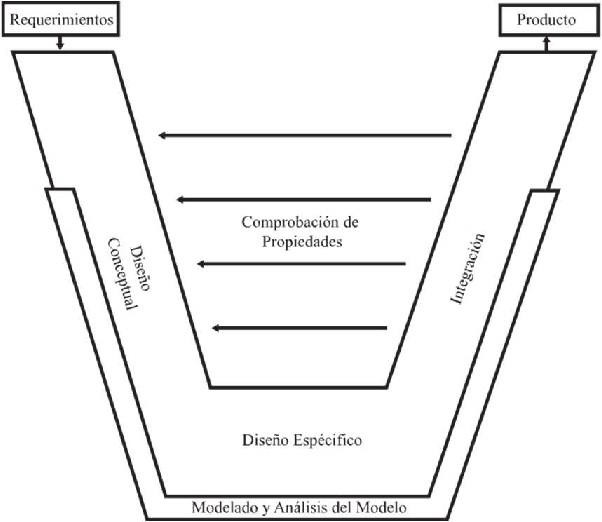
\includegraphics[width=0.7\linewidth]{imagenes/imacap/marcoteo/VDI2206.jpeg}
    \caption{Metodología "V" para el desarrollo del proyecto}
    \label{fig:MetodologiaV}
\end{figure}

%%%%%%fin del archivo
\endinput 